Viene ora presentata, invece, la versione completa e finale del progetto. Anche qui, come nel caso precedente, si inizia con un modello senza posti monitor. Tale modello è presentato in Fig. \ref{fig:semafori_finale}.

\begin{figure}[ht]
    \centering
    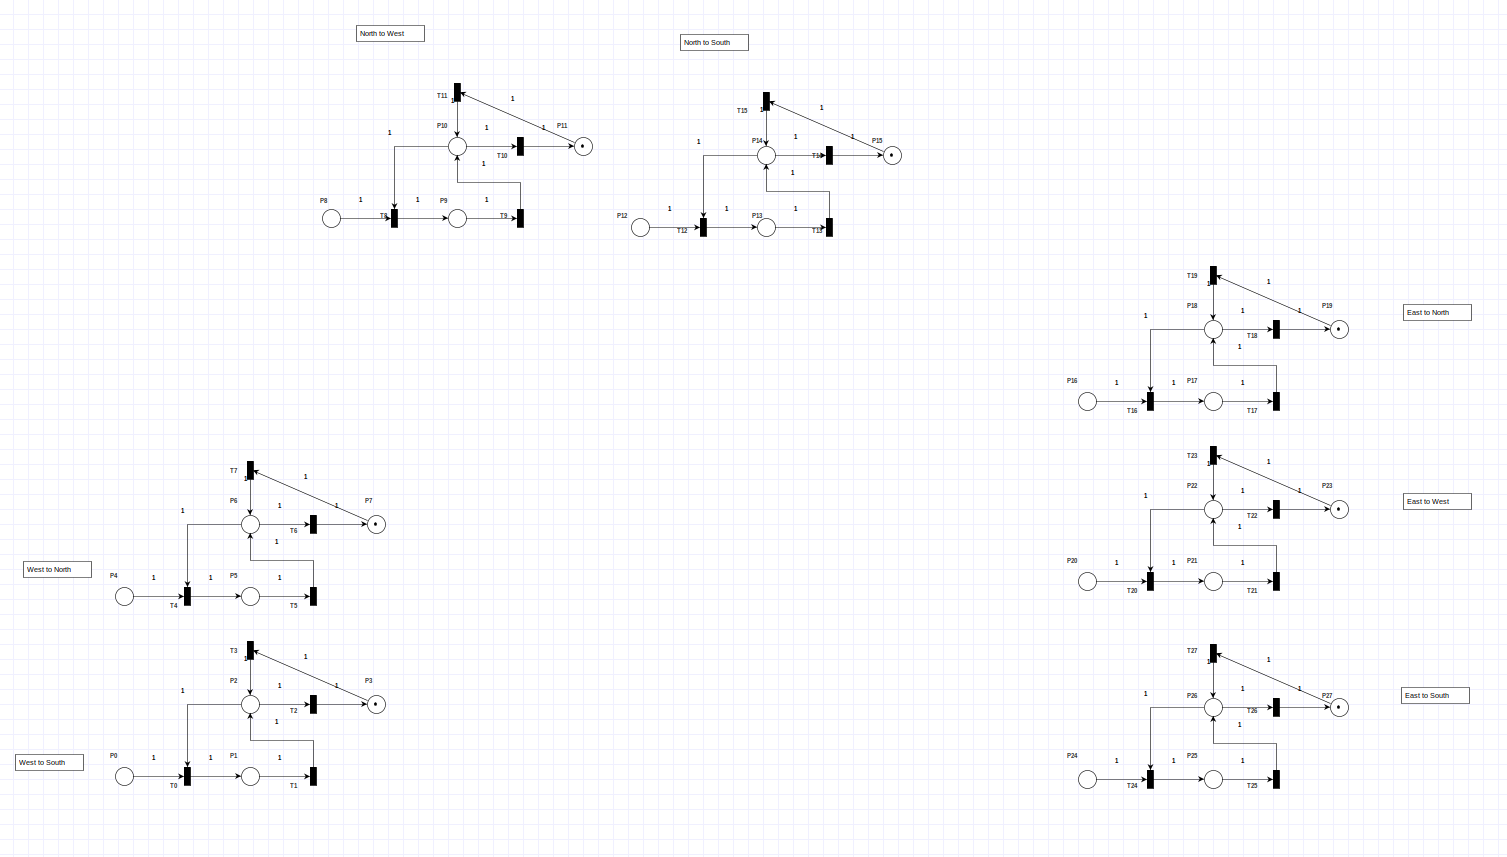
\includegraphics[width=0.8\textwidth]{figure/project_screenshots/semafori_finale.png}
    \caption{Modello finale senza controlli}
    \label{fig:semafori_finale}
\end{figure}

Appare subito evidente, quindi, come questo sia semplicemente una ripetizione del semaforo visto nella sezione \ref{sec:3.1}. Sono state inoltre aggiunte alcune etichette per fare chiarezza sulla direzione di provenienza e di destinazione dei veicoli.

Si procede, dunque, con l'implenentare tutti i vincoli richiesti come dettagliati nella sezione successiva. Il modello finale, con i posti monitor, è presentato in Fig. \ref{fig:semafori_finale_monitor}. Tale modello impedisce che due veicoli si incrocino all'interno dell'incrocio, come ad esempio un veicolo che attraversa l'incrocio da Est a Ovest e un veicolo che attraversa l'incrocio da Nord a Sud. Inoltre, non è possibile attraversare contemporaneamente l'incrocio con due veicoli provenienti da direzioni diverse e diretti nella stessa direzione, in quanto ciò potrebbe causare un incidente.

\begin{figure}[htb]
    \centering
    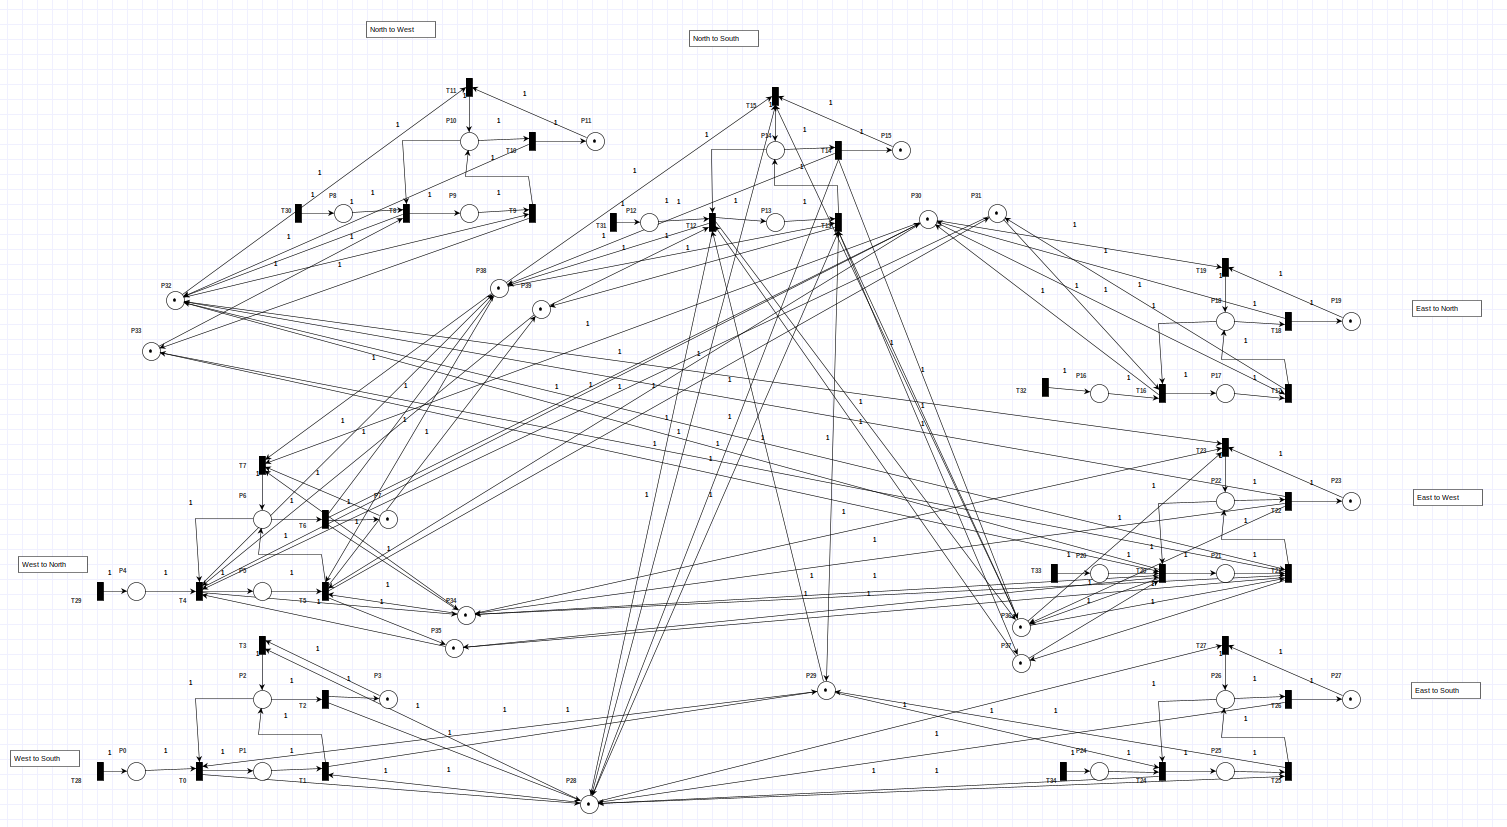
\includegraphics[width=1.0\textwidth]{figure/project_screenshots/semafori_finale_2.png}
    \caption{Modello finale con controlli}
    \label{fig:semafori_finale_monitor}
\end{figure}